\documentclass[12pt,a4paper]{report}



\usepackage{geometry}
\geometry{margin=0.8in}


\usepackage[latin1]{inputenc}
\usepackage{amsmath}
\usepackage{algorithmicx}
\usepackage{algpseudocode}
\usepackage{amsfonts}
\usepackage{amssymb}
\usepackage{graphicx}
\author{Yimin}
\title{optimization}
\begin{document}
	
\section{Equation}
\begin{eqnarray}
-\nabla D \nabla u + \sigma_a u = f \\
2D\frac{\partial u}{\partial n} + u = 0
\end{eqnarray}
where $D = 1/(3\sigma_t)$, $\sigma_t = \sigma_a + \sigma_s$, the weak form 
\begin{eqnarray}
\int (D\nabla u \nabla v + \sigma_a u v)\mathrm{d}x  + \frac{1}{2}\int_{\partial} uv \mathrm{d} s= \int f v \label{eq:3}
\end{eqnarray}

\section{Numerical Experiment}
\subsection{single internal data $H = u$}
according to (\ref{eq:3}), the finite element space solution $U$ satisfies
\begin{eqnarray}
A U = F \label{eq:4}
\end{eqnarray}
and $A_{ij} = \int D\nabla\psi_i \nabla\psi_j + \int\sigma_a \psi_i \psi_j + \frac{1}{2}\int_{\partial} \psi_i \psi_j$, $F_j = \int f\psi_j$. Differentiate (\ref{eq:4}),
\begin{eqnarray}
\frac{\partial A}{\partial\sigma_a} U + A\frac{\partial U}{\partial \sigma_a} = 0
\end{eqnarray}

\begin{eqnarray}
\frac{\partial U}{\partial \sigma_a} = -A^{-1} \frac{\partial A}{\partial \sigma_a} U
\end{eqnarray}
where $\frac{\partial A}{\partial \sigma_a}$ is linear operator $\mathbb{R}^{m\times n \times n}\to \mathbb{R}^{m\times n}$.

\subsubsection{objective function without regularization}
\begin{eqnarray}
f(U) = \frac{1}{2}\int (U - H)^2
\end{eqnarray}
suppose $M$ is mass matrix, then
\begin{eqnarray}
\frac{\partial f}{\partial \sigma_a} =  (U - H)^{T} M \frac{\partial U}{\partial \sigma_a} = -(U - H)^T M A^{-1}\frac{\partial A}{\partial \sigma_a}U 
\end{eqnarray}
taking the adjoint,
\begin{eqnarray}
\frac{\partial f}{\partial \sigma_a} = -U^{T} \frac{\partial A}{\partial \sigma_a}^T A^{-T} M^T(U-H)
\end{eqnarray}
due to symmetric property of $M$ and $A$, it is straightforward to write as
\begin{eqnarray}
\frac{\partial f}{\partial \sigma_a} = -U^{T} \frac{\partial A}{\partial \sigma_a} \underline{A^{-1} M (U-H)} \label{eq:10}
\end{eqnarray}
\subsubsection{Result}
\begin{itemize}
\item domain $[0, 1]\times [0, 1]$, element size $1/40$.
\item source $f(x) = \chi_{r < |x - x_0| < R}$
\item $\sigma_s = 20$ as constant, $\sigma_a = 0.1$ as true value
\item $\sigma_s$ and $\sigma_a$ are piecewise constant function.
\item relative error calculated from $\|\sigma_a - \tilde{\sigma}_a\|/\|\sigma_a\|$
\item initial value for BFGS $\sigma_{a0} = 0.06$ throughout domain.
\item No regularization required.
\end{itemize}

\begin{figure}[htb]
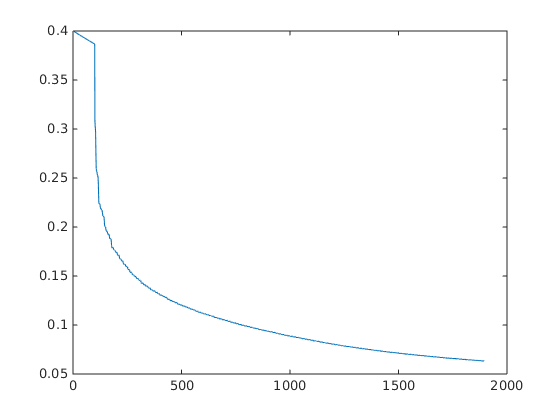
\includegraphics{sigma_a_rate}
\caption{Relative error of $\sigma_a$ with respect to iteration number}
\end{figure}
\begin{itemize}
\item The iteration continues to around 15000, and the final objective function can reach less than machine error(1e-19).
\item The relative error on $\sigma_a$ observed from the graph above is $6\%$.
\item The converging rate is almost linear after 2000 iterations, but slow. 
\end{itemize}

\begin{figure}[htb]
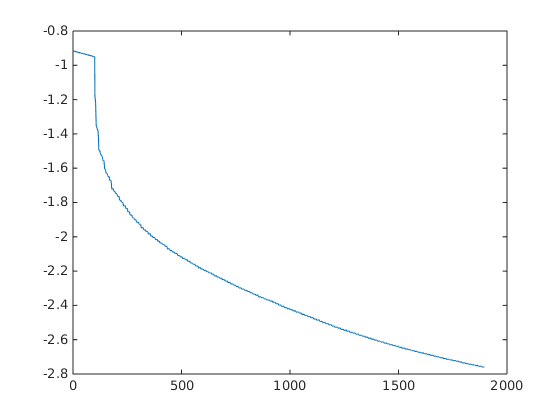
\includegraphics{log_sigma_a_rate}
\caption{Log of relative error of $\sigma_a$ with respect to iteration number}
\end{figure}
\begin{figure}[htb!]
	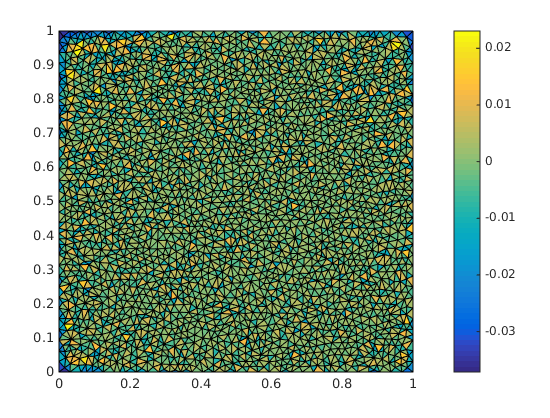
\includegraphics{error_2d_sigma_a}
	\caption{Absolute error of $\sigma_a$}
\end{figure}
\begin{figure}[htb!]
	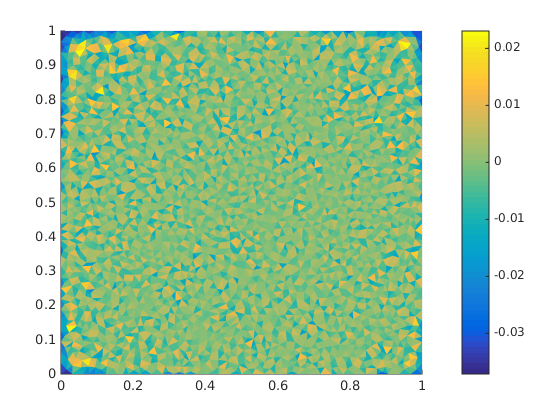
\includegraphics{error_2d_sigma_a_no_edge}
	\caption{Absolute error of $\sigma_a$}
\end{figure}
\begin{itemize}
\item The absolute error is large on corners, the relative $L^{\infty}$ error is over $30\%$.
\item The absolute error in center is much more better.
\end{itemize}
\begin{figure}[htb!]
	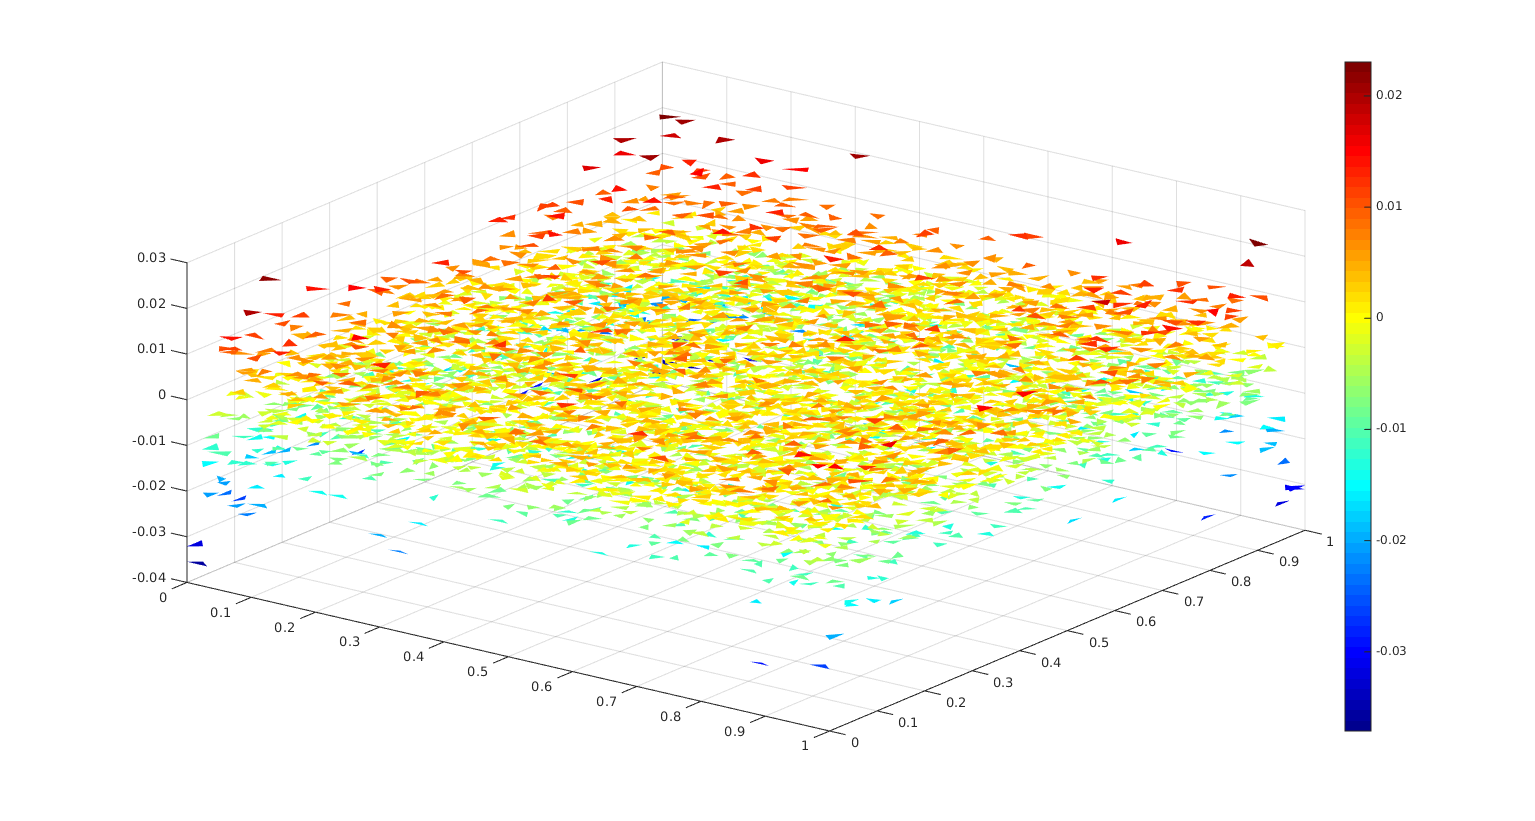
\includegraphics[scale = 0.5]{error_2d_sigma_a_colormap_jet}
	\caption{3D view of absolute error of $\sigma_a$}
\end{figure}
\newpage
\subsubsection{objective function with regularization}
\begin{eqnarray}
f(U) = \int (U- H)^2 + \alpha R (\sigma_a)
\end{eqnarray}
where $R(\sigma_a)$ is calculated through following algorithm

\begin{center}
\begin{algorithmic}
	\For {$1\leq i\leq nelem$}
	\For {$j$ is $i$'s neighbor}
	\State $R \gets R + (\sigma_a(i) - \sigma_a(j))^2$
	\EndFor
	\EndFor
\end{algorithmic}
\end{center}

\subsubsection{result}
\begin{itemize}
	\item Regularization parameter $\alpha = 1e-8$
	\item other settings are the same as previous settings
\end{itemize}

\begin{itemize}
	\item After regularization, relative error gets to $1.19\%$, after 150 iterations.
\end{itemize}
\begin{figure}[htb!]
	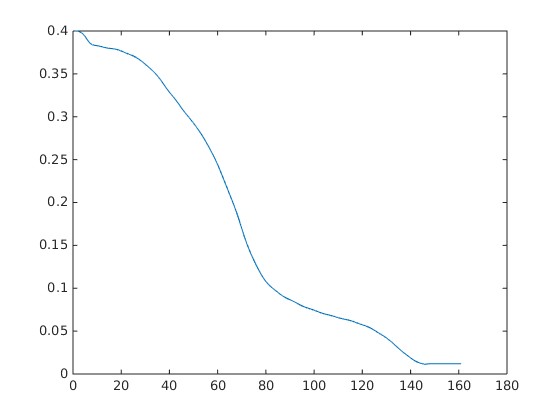
\includegraphics{sigma_a_rate_reg}
	\caption{relative error of $\sigma_a$ with respect to iteration number with regularization}
\end{figure}
\begin{figure}[htb!]
	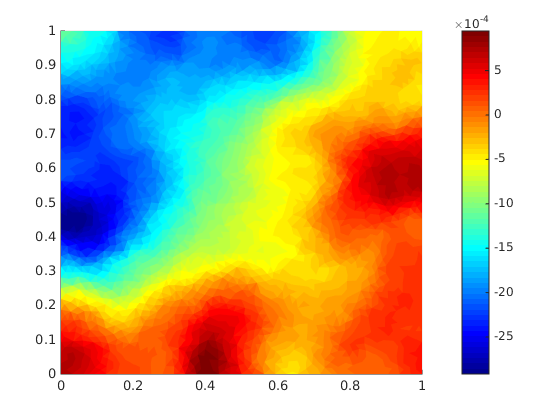
\includegraphics{error_2d_reg}
	\caption{absolute error of regularized case}
\end{figure}

\begin{figure}[htb!]
	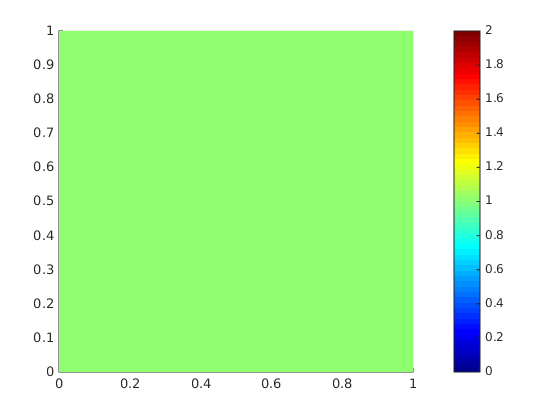
\includegraphics{true}
	\caption{true constant $\sigma_a$}
\end{figure}

\begin{figure}[htb!]
	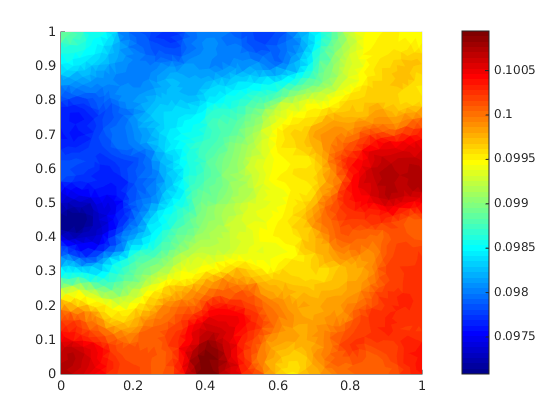
\includegraphics{recovered}
	\caption{recovered $\sigma_a$}
	\end{figure}
		
\subsection{More cases}
\begin{figure}[htb!]
	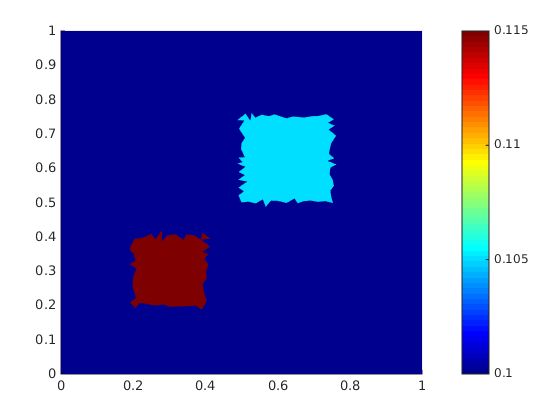
\includegraphics{two_blocks}
	\caption{Two square blocks, true $\sigma_a$}
\end{figure}
\begin{figure}[htb!]
	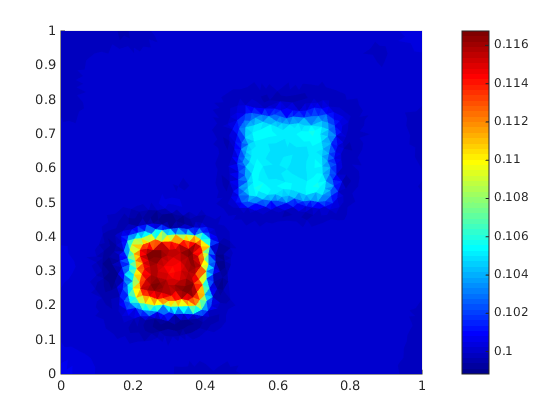
\includegraphics{recovered_two_block}
	\caption{Recovered two square blocks $\sigma_a$, error less than $0.94\%$}
\end{figure}

\begin{figure}[htb!]
	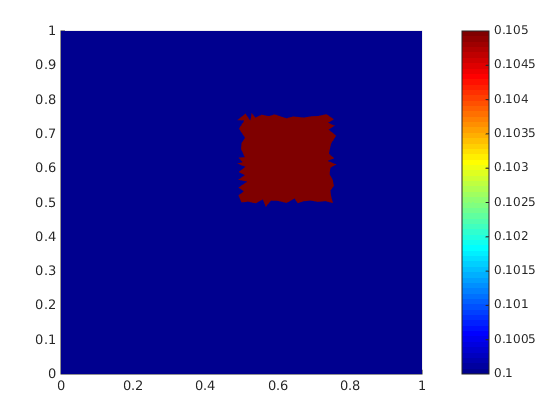
\includegraphics{discont_real}
	\caption{Single block discontinuous, true $\sigma_a$}
\end{figure}
\begin{figure}[htb!]
	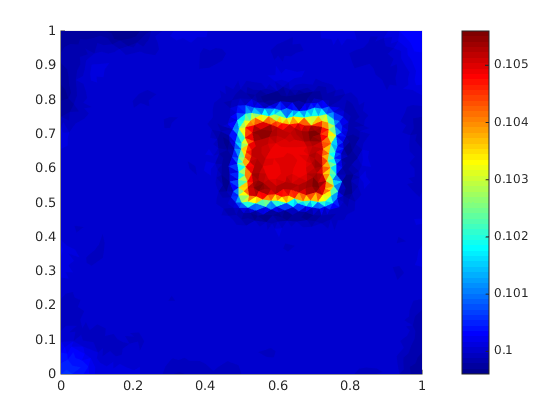
\includegraphics{discont_recover}
	\caption{Recovered single block $\sigma_a$, error less than $0.35\%$}
\end{figure}

\end{document}